\documentclass{article}
\usepackage[letterpaper,noheadfoot,dvips,pdftex]{geometry}
\usepackage{graphicx}

\begin{document}

\title{\texttt{fragmaster.pl} test document}
\author{Tilman Vogel}

\maketitle

This document includes graphics generated by \texttt{fragmaster.pl}.

\begin{center}
  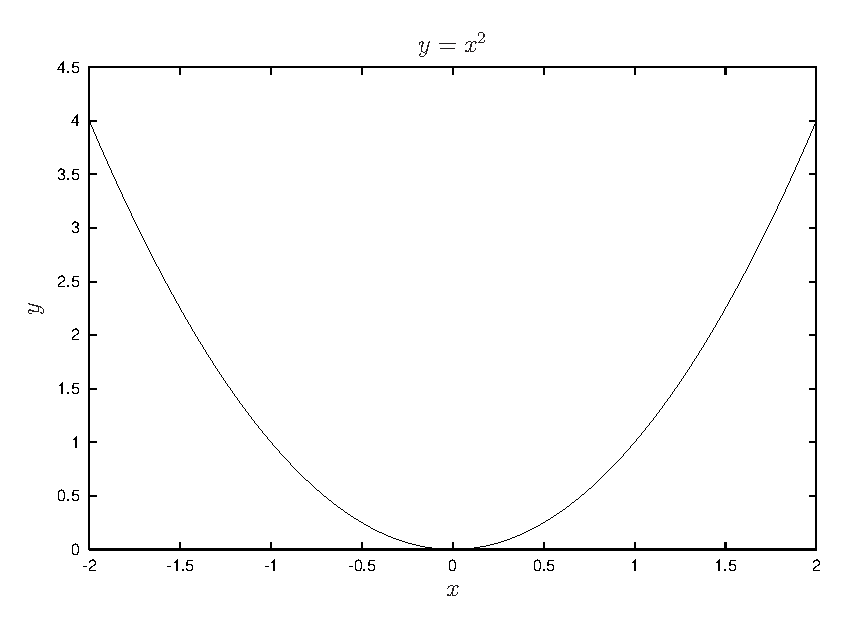
\includegraphics[width=0.6\textwidth]{parabel}
\end{center}

The title and the labels for the $x$ and $y$ axis have been replaced
with \LaTeX\ code using \texttt{psfrag}. The original graphics was:

\begin{center}
  \includegraphics[width=0.6\textwidth]{parabel_fm}
\end{center}

The document can be processed both by \texttt{latex} and
\texttt{pdflatex}.

\end{document}

%%% Local Variables: 
%%% mode: latex
%%% TeX-master: t
%%% End: 
